
In a 2D Cartesian domain overlain by a $nnx \times nny$ grid, 
the spacing between nodes in the $x$ and $y$ direction is $h_x$ 
and $h_y$ respectively. 

\begin{center}


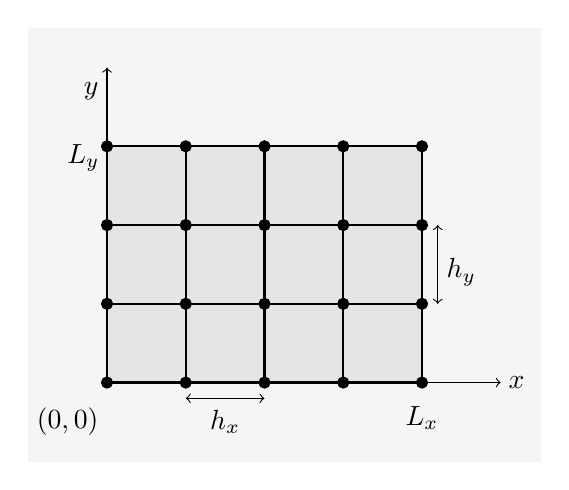
\begin{tikzpicture}
\draw[fill=gray!8,gray!8](0,0) rectangle (6.5,5.5);
%\draw[step=0.5cm,gray,very thin] (0,0) grid (8,5); %background grid


\draw[fill=gray!20,gray!20](1,1) rectangle (5,4);
\draw[thick] (1,1) -- (5,1) -- (5,4) -- (1,4) -- cycle;  

\draw[thick] (1,2) -- (5,2) ; 
\draw[thick] (1,3) -- (5,3) ; 
\draw[thick] (2,1) -- (2,4) ; 
\draw[thick] (3,1) -- (3,4) ; 
\draw[thick] (4,1) -- (4,4) ; 

\draw[black,fill=black] (1,1)  circle (2pt);
\draw[black,fill=black] (2,1)  circle (2pt);
\draw[black,fill=black] (3,1)  circle (2pt);
\draw[black,fill=black] (4,1)  circle (2pt);
\draw[black,fill=black] (5,1)  circle (2pt);
\draw[black,fill=black] (1,2)  circle (2pt);
\draw[black,fill=black] (2,2)  circle (2pt);
\draw[black,fill=black] (3,2)  circle (2pt);
\draw[black,fill=black] (4,2)  circle (2pt);
\draw[black,fill=black] (5,2)  circle (2pt);
\draw[black,fill=black] (1,3)  circle (2pt);
\draw[black,fill=black] (2,3)  circle (2pt);
\draw[black,fill=black] (3,3)  circle (2pt);
\draw[black,fill=black] (4,3)  circle (2pt);
\draw[black,fill=black] (5,3)  circle (2pt);
\draw[black,fill=black] (1,4)  circle (2pt);
\draw[black,fill=black] (2,4)  circle (2pt);
\draw[black,fill=black] (3,4)  circle (2pt);
\draw[black,fill=black] (4,4)  circle (2pt);
\draw[black,fill=black] (5,4)  circle (2pt);

\draw [<->] (5.2,2) -- (5.2,3); \node[] at (5.5,2.4) {$h_y$};
\draw [<->] (2,0.8) -- (3,0.8); \node[] at (2.5,0.5) {$h_x$};

\draw [->] (5,1) -- (6,1); \node[] at (6.2,1) {$x$};
\draw [->] (1,4) -- (1,5); \node[] at (0.8,4.7) {$y$};

\node[] at (0.5,0.5) {$(0,0)$};
\node[] at (5,0.55) {$L_x$};
\node[] at (0.7,3.85) {$L_y$};

%\node[] at (2.2,3.1) {\tiny{\color{brown}i-1,j}};
%\node[] at (3.2,3.1) {\tiny{\color{brown}i,j}};
%\node[] at (4.2,3.1) {\tiny{\color{brown}i+1,j}};

%\node[] at (3.2,4.1) {\tiny{\color{brown}i,j+1}};
%\node[] at (3.2,2.1) {\tiny{\color{brown}i,j-1}};

%\draw[black,fill=black] (3.1,0.2) circle (2pt); \node[] at (3.4,0.2) {$\vec\upnu$};
%\draw (4.1,0.2) circle (4pt); 
%\node[] at (2.5,4.5) {4 vel. nodes, 1 press. nodes};
\end{tikzpicture}

\end{center}

We have seen in Section~\ref{ss:fdm_basics1D} how to discretise second-order derivatives in 1D. 
In 2D, we then logically have for a function $f(x,y)$

\begin{equation}
\frac{\partial^2 f}{\partial x^2}(x_0,y_0) = \frac{f(x_0+h_x,y_0) -2f(x_0,y_0) + f(x_0-h_x,y_0) }{h_x^2} 
+ {\cal O}(h_x^2)
\end{equation}
\begin{equation}
\frac{\partial^2 f}{\partial y^2}(x_0,y_0) = \frac{f(x_0,y_0+h_y) -2f(x_0,y_0) + f(x_0,y_0-h_y) }{h_y^2} 
+ {\cal O}(h_y^2)
\end{equation}
What about mixed derivatives? Since these are combinations of first-order derivatives, 
we can straightforwardly discretise them:
\begin{eqnarray}
&& \frac{\partial^2 f }{\partial x \partial y}(x_0,y_0) \nn\\
&=& \frac{\partial }{\partial x} \left(\frac{\partial f}{\partial y}\right) (x_0,y_0) \nn\\
&=& \frac{\partial }{\partial x} \left(\frac{ f(x_0,y_0+h_y)-f(x_0,y_0-h_y)}{2h_y} \right) \nn\\
&=& \frac{1}{2h_y} \frac{\partial f}{\partial x} (x_0,y_0+h_y)
   -\frac{1}{2h_y} \frac{\partial f}{\partial x} (x_0,y_0-h_y) \nn\\
&=& \frac{1}{2h_y}  \frac{ f(x_0+h_x,y_0+h_y)-f(x_0-h_x,y_0+h_y)}{2h_x} 
-   \frac{1}{2h_y}  \frac{ f(x_0+h_x,y_0-h_y)-f(x_0-h_x,y_0-h_y)}{2h_x}  \nn\\
&=& \frac{f(x_0+h_x,y_0+h_y)-f(x_0-h_x,y_0+h_y)-f(x_0+h_x,y_0-h_y)+f(x_0-h_x,y_0-h_y)}{2 h_x h_y}
+ {\cal O}(h_x^2,h_y^2) \nn
\end{eqnarray}

%...............................
\subsubsection{From 1D to 2D}

INSERT TEXT

\begin{center}
\begin{flushright} {\tiny {\color{gray} (tikz\_needicon.tex)}} \end{flushright}
%~~~~~~~~~~~~~~~~~~~~~~~~~~~~~~~~~~~~~~~~~~~~~~~~~~~~~~~~~~~~~~~~~~~~~~~~~~~~~~~~~~~~~~~~~~~~~~~~~~


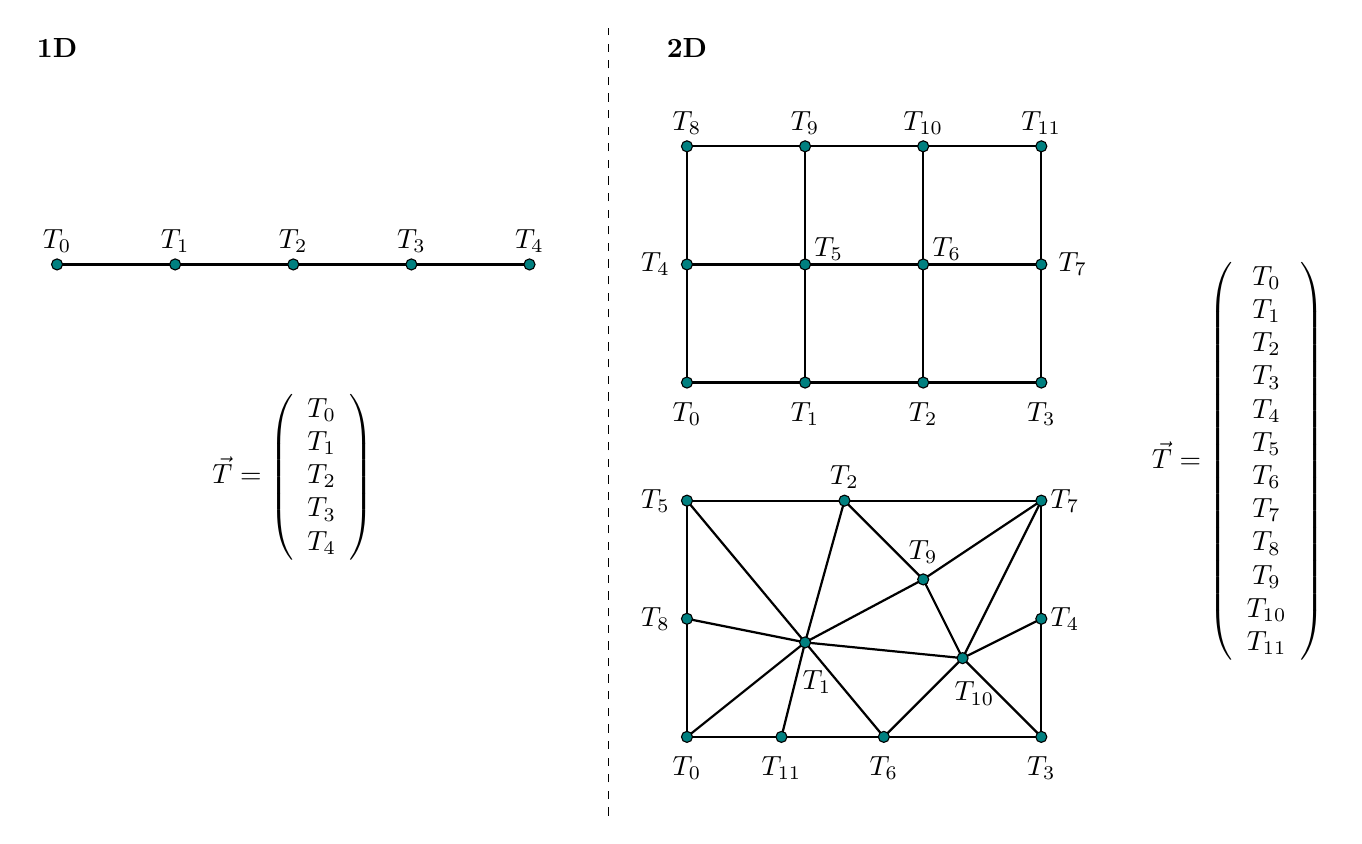
\begin{tikzpicture}
%\draw[step=0.5cm,gray,very thin] (0,0) grid (17,10); 

\node[] at (1,9.75) {\bf 1D};

\draw[thick] (1,7)--(7,7);
\draw[black,fill=teal] (1,7) circle (2pt);
\draw[black,fill=teal] (2.5,7) circle (2pt);
\draw[black,fill=teal] (4,7) circle (2pt);
\draw[black,fill=teal] (5.5,7) circle (2pt);
\draw[black,fill=teal] (7,7) circle (2pt);

\node[] at (1,7.3) {$T_0$};
\node[] at (2.5,7.3) {$T_1$};
\node[] at (4,7.3) {$T_2$};
\node[] at (5.5,7.3) {$T_3$};
\node[] at (7,7.3) {$T_4$};

\node[] at (4,4.3) {
$\vec{T}=\left(
\begin{array}{c}
T_0 \\ T_1 \\ T_2 \\ T_3 \\ T_4
\end{array}
\right)$};

%%%%%%%%%%%%%%%%%%%%%%%%%%%%%%%%%%%%%%%%%55
\draw[dashed] (8,0)--(8,10); 

\node[] at (9,9.75) {\bf 2D};

\draw[thick](9,5.5) rectangle (13.5,8.5);
\draw[thick](9,7)--(13.5,7);
\draw[thick](10.5,5.5)--(10.5,8.5);
\draw[thick](12,5.5)--(12,8.5);

\node[] at (16,4.5) {
$\vec{T}=\left(
\begin{array}{c}
T_0 \\ T_1 \\ T_2 \\ T_3 \\ T_4 \\
T_5 \\ T_6 \\ T_7 \\ T_8 \\ T_9 \\ T_{10} \\ T_{11}
\end{array}
\right)$};

\draw[black,fill=teal] (9,5.5) circle (2pt);
\draw[black,fill=teal] (10.5,5.5) circle (2pt);
\draw[black,fill=teal] (12,5.5) circle (2pt);
\draw[black,fill=teal] (13.5,5.5) circle (2pt);

\draw[black,fill=teal] (9,7) circle (2pt);
\draw[black,fill=teal] (10.5,7) circle (2pt);
\draw[black,fill=teal] (12,7) circle (2pt);
\draw[black,fill=teal] (13.5,7) circle (2pt);

\draw[black,fill=teal] (9,8.5) circle (2pt);
\draw[black,fill=teal] (10.5,8.5) circle (2pt);
\draw[black,fill=teal] (12,8.5) circle (2pt);
\draw[black,fill=teal] (13.5,8.5) circle (2pt);

\node[] at (9,5.1) {$T_0$};
\node[] at (10.5,5.1) {$T_1$};
\node[] at (12,5.1) {$T_2$};
\node[] at (13.5,5.1) {$T_3$};
\node[] at (8.6,7) {$T_4$};

\node[] at (10.8,7.2) {$T_5$};
\node[] at (12.3,7.2) {$T_6$};

\node[] at (13.9,7) {$T_7$};

\node[] at (9,8.8) {$T_8$};
\node[] at (10.5,8.8) {$T_9$};
\node[] at (12,8.8) {$T_{10}$};
\node[] at (13.5,8.8) {$T_{11}$};

%%%%%%%%%%%%%%%%%%%%%%%%%%%%%%%%%%%%%%%5
%triangular mesh

\draw[thick](9,1) rectangle (13.5,4);


\draw[thick](9,1)--(10.5,2.2)--(12,3)--(13.5,4);
\draw[thick](9,4)--(10.5,2.2)--(12.5,2)--(13.5,1);
\draw[thick](11,4)--(12,3)--(12.5,2)--(13.5,2.5);
\draw[thick](13.5,4)--(12.5,2)--(11.5,1)--(10.5,2.2)--(9,2.5);
\draw[thick](10.2,1)--(10.5,2.2)--(11,4);


\draw[black,fill=teal] (9,1) circle (2pt);
\draw[black,fill=teal] (10.2,1) circle (2pt);
\draw[black,fill=teal] (11.5,1) circle (2pt);
\draw[black,fill=teal] (13.5,1) circle (2pt);

\draw[black,fill=teal] (9,2.5) circle (2pt);
\draw[black,fill=teal] (10.5,2.2) circle (2pt);
\draw[black,fill=teal] (12,3) circle (2pt);
\draw[black,fill=teal] (12.5,2) circle (2pt);
\draw[black,fill=teal] (13.5,2.5) circle (2pt);

\draw[black,fill=teal] (9,4) circle (2pt);
\draw[black,fill=teal] (11,4) circle (2pt);
\draw[black,fill=teal] (13.5,4) circle (2pt);

\node[] at (9,0.6) {$T_0$};
\node[] at (10.2,0.6) {$T_{11}$};
\node[] at (11.5,0.6) {$T_6$};
\node[] at (13.5,0.6) {$T_3$};

\node[] at (8.6,2.5) {$T_8$};
\node[] at (8.6,4) {$T_5$};
\node[] at (11,4.3) {$T_2$};
\node[] at (13.8,4) {$T_7$};
\node[] at (13.8,2.5) {$T_4$};

\node[] at (12,3.35) {$T_9$};
\node[] at (12.65,1.55) {$T_{10}$};

\node[] at (10.65,1.7) {$T_1$};

\end{tikzpicture}

\end{center}


Also, here is a rather handy code snippet which should allow you to make nice plots of the coming exercises.

\begin{lstlisting}
       filename = 'solution_{:04d}.pdf'.format(istep) 
       fig = plt.figure ()
       ax = fig.gca(projection='3d')
       ax.plot_surface(x.reshape ((nny,nnx)),y.reshape((nny,nnx)),T.reshape((nny,nnx)),color = 'darkseagreen')
       ax.set_xlabel ( 'X [ m ] ')
       ax.set_ylabel ( 'Y [ m ] ')
       ax.set_zlabel ( ' Temperature  [ C ] ')
       plt.title('Timestep  %.2d' %(istep),loc='right')
       plt.grid ()
       plt.savefig(filename)
       #plt.show ()
       plt.close()
\end{lstlisting}

